%%%%%%%%%%%%%%%%%%%%%%%%%%%%%%%%%%%%%%%%%%%%%%%%%%%%%%%%%%%%%%%%%%%%%%%%%
 
\begin{figure}[p]
\begin{center}
\begin{tabular}{cc}
  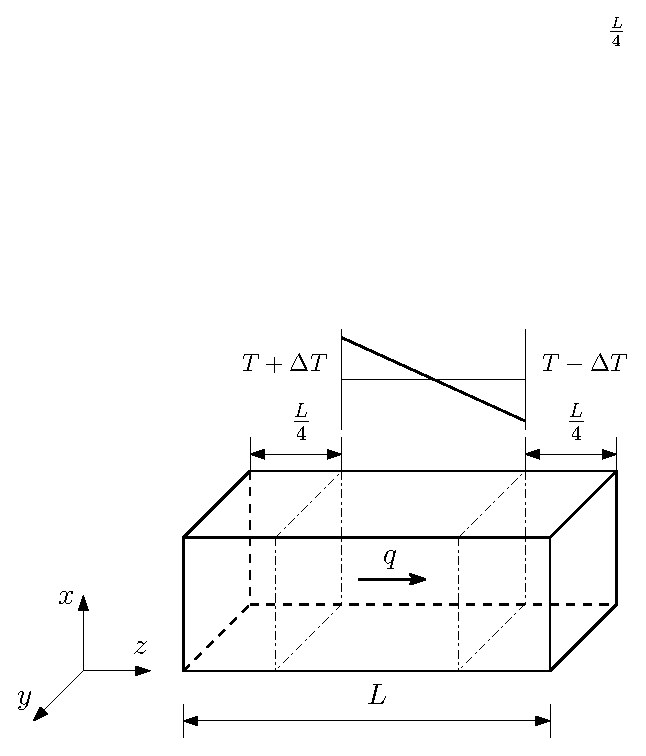
\includegraphics[width=0.48\textwidth]{./Figures/schematic}
  &
  \hspace{3mm}
  \includegraphics[width=0.40\textwidth]{./Figures/Sibar_05}
  \\ (a) & (b)
  \end{tabular}
\caption{(a) Schematic illustration of the set-up for evaluating thermal conductivity of Si using NEMD. (b) 
Arrangement of Si atoms prior to the application of thermal gradient.}
\label{fig:setup}
\end{center}
\end{figure}

\clearpage

%%%%%%%%%%%%%%%%%%%%%%%%%%%%%%%%%%%%%%%%%%%%%%%%%%%%%%%%%%%%%%%%%%%%%%%%%

\begin{figure}[p]
 \begin{center}
  \includegraphics[width=0.70\textwidth]{./Figures/temp_plot}
\caption{Temperature distribution along a Si bar of length 14.74~nm for different scenarios of applied 
thermal gradient.}
\label{fig:kapitza}
\end{center}
\end{figure}


\clearpage

%%%%%%%%%%%%%%%%%%%%%%%%%%%%%%%%%%%%%%%%%%%%%%%%%%%%%%%%%%%%%%%%%%%%%%%%%

\begin{figure}[p]
\begin{center}
\begin{tabular}{cc}
  \hspace{-12mm}
  \includegraphics[width=0.60\textwidth]{./Figures/realz_quad300K}
  &
  \hspace{-9mm}
  \includegraphics[width=0.56\textwidth]{./Figures/PCspectrum_300}
  \\ (a) & (b)
  \end{tabular}
\caption{(a) Realizations of discrepancy in bulk thermal conductivity at the Gauss-Legendre quadrature notes are
depicted using circles. The size of the circle in each case is proportional to the discrepancy estimate, also provided
 in cases where it is observed to be relatively large. (b) Spectrum of PC coefficients is depicted using circles of
 varying sizes, proportional to the log value of their magnitude. The computations were performed at 300 K.}
\label{fig:rs1}
\end{center}
\end{figure}

\clearpage

%%%%%%%%%%%%%%%%%%%%%%%%%%%%%%%%%%%%%%%%%%%%%%%%%%%%%%%%%%%%%%%%%%%%%%%%%

\begin{figure}[p]
\begin{center}
\begin{tabular}{cc}
 \hspace{-10mm}
  \includegraphics[width=0.55\textwidth]{./Figures/err2D_300}
  &
  %\hspace{-9mm}
  \includegraphics[width=0.55\textwidth]{./Figures/err2D_500}
  \\ (a) & (b)
  \end{tabular}
  \\ \vspace{1mm}
  \includegraphics[width=0.50\textwidth]{./Figures/err2D_s}
  \\ (c)
\caption{Response surface of the discrepancy in bulk thermal conductivity at (a) $T$ = 300~K and
 (b) $T$ = 500~K. Gauss-Legendre quadrature nodes are highlighted in both cases. (c) Sobol samples
 in the 2D domain used for verifying the accuracy of the response surfaces.}
\label{fig:rs2}
\end{center}
\end{figure}

\clearpage

%%%%%%%%%%%%%%%%%%%%%%%%%%%%%%%%%%%%%%%%%%%%%%%%%%%%%%%%%%%%%%%%%%%%%%%%%

\begin{figure}[p]
\begin{center}
\begin{tabular}{cc}
 \hspace{-10mm}
  \includegraphics[width=0.50\textwidth]{./Figures/kinv_300}
  &
  %\hspace{-9mm}
  \includegraphics[width=0.50\textwidth]{./Figures/kinv_500}
  \\ (a) & (b)
  \end{tabular}
 \caption{Inverse of the bulk thermal conductivity estimates are plotted against the inverse of Si bar length
 using predictions from NEMD as well as estimates from the response surface at (a)  $T$ = 300~K and 
 (b) $T$ = 500~K.}
\label{fig:rs3}
\end{center}
\end{figure}

\clearpage

%%%%%%%%%%%%%%%%%%%%%%%%%%%%%%%%%%%%%%%%%%%%%%%%%%%%%%%%%%%%%%%%%%%%%%%%%


